\documentclass[11pt,a4paper]{article}

% Pakiety
\usepackage{iftex}
\ifXeTeX
  \usepackage{fontspec} % XeTeX/Tectonic: czcionki Unicode (domyślnie Latin Modern)
\else
  \usepackage[utf8]{inputenc}
  \usepackage[T1]{fontenc}
  \usepackage{lmodern}
\fi
\usepackage[polish]{babel}
\usepackage{xcolor}
\usepackage[a4paper,margin=2.3cm,headheight=14pt]{geometry}
\usepackage{amsmath,amssymb,amsthm,mathtools}
\usepackage{graphicx}
\usepackage{booktabs}
\usepackage{listings}
\usepackage{algorithm}
\usepackage[noEnd=true]{algpseudocodex}
\usepackage[font=small,labelfont=normal]{caption}
\usepackage{fancyhdr}
\usepackage{titlesec}
\usepackage{microtype}

% Układ strony: nagłówek po prawej, numer strony na dole
\pagestyle{fancy}
\fancyhf{}
\fancyhead[R]{\small Rekurencyjne odwracanie macierzy i faktoryzacja LU}
\fancyfoot[C]{\thepage}
\renewcommand{\headrulewidth}{0pt}
\fancypagestyle{plain}{\fancyhf{}\fancyfoot[C]{\thepage}\renewcommand{\headrulewidth}{0pt}}

% Akapity i nagłówki sekcji (pogrubione, bezszeryfowe)
\setlength{\parindent}{1.5em}
\setlength{\parskip}{2pt}
\titleformat{\section}{\Large\bfseries\sffamily}{\thesection}{1em}{}
\titleformat{\subsection}{\large\bfseries\sffamily}{\thesubsection}{1em}{}
\titlespacing*{\section}{0pt}{16pt}{8pt}
\titlespacing*{\subsection}{0pt}{12pt}{6pt}
\renewcommand{\arraystretch}{1.1}

% Styl fragmentów kodu C++
\lstset{
  language=C++,
  basicstyle=\ttfamily\scriptsize,
  keywordstyle=\bfseries,
  commentstyle=\itshape\color[gray]{0.35},
  numbers=left, numberstyle=\tiny, numbersep=4pt,
  frame=single, framerule=0.3pt, rulecolor=\color[gray]{0.6},
  xleftmargin=10pt, aboveskip=3pt, belowskip=3pt,
  columns=fullflexible, keepspaces=true, showstringspaces=false
}

% Pseudokod: polskie słowa kluczowe
\floatname{algorithm}{Algorytm}
\algrenewcommand\algorithmicprocedure{\textbf{Procedura}}
\algrenewcommand\algorithmicif{\textbf{Jeżeli}}
\algrenewcommand\algorithmicthen{\textbf{wykonaj}}
\algrenewcommand\algorithmicelse{\textbf{W przeciwnym razie}}
\algrenewcommand\algorithmicreturn{\textbf{Zwróć}}

\newcommand{\Pomnoz}{\textsc{Pomnóż}}
\newcommand{\Odwroc}{\textsc{Odwróć}}

% Twierdzenia i dowody
\newtheorem{tw}{Twierdzenie}
\newtheorem{lem}{Lemat}
\renewcommand{\proofname}{Dowód}

% Miejsca do uzupełnienia (widoczne w PDF na czerwono)
\newcommand{\todo}[1]{\textcolor{red}{\textbf{[DO UZUPEŁNIENIA: #1]}}}

\begin{document}

% STRONA TYTUŁOWA + SPIS TREŚCI
\thispagestyle{plain}
\begin{center}
\vspace*{3.5cm}
{\Large Rekurencyjne odwracanie macierzy i faktoryzacja LU}\\[1.5em]
Mateusz Majta, Maksymilian Siemek\\[1.2em]
Algorytmy Macierzowe 2026/2027, grupa 2
\end{center}
\vspace{1.2cm}
\tableofcontents
\newpage

% 1. WSTĘP
\section{Wstęp}
Celem ćwiczenia była implementacja rekurencyjnego odwracania macierzy z mnożeniem metodami Binét'a, Strassena
i Ladermana oraz rekurencyjnej faktoryzacji LU z mnożeniem metodami Binét'a i Strassena. Wszystkie algorytmy działają
dla macierzy kwadratowych $n\times n$ o dowolnym rozmiarze, a macierze testowe zawierają liczby losowe z rozkładu
równomiernego na przedziale $(10^{-8}, 1)$. Macierze mnożymy algorytmami z zadania~1, uogólnionymi na macierze
prostokątne (rozdział~\ref{sec:mnozenie}). Rekurencyjne mnożenie metodą Ladermana (punkt~4 zestawu) wykonaliśmy
w zadaniu~1. Liczymy wszystkie operacje zmiennoprzecinkowe $+,-,*,/$ na liczbach.

Kod w C++ jest w folderze \texttt{task2}: \texttt{common.hpp} (macierz, licznik operacji), \texttt{mul\_*.hpp}
(metody mnożenia), \texttt{inverse.hpp}/\texttt{inverse.cpp} (odwracanie), \texttt{lu.hpp}/\texttt{lu.cpp}
(faktoryzacja LU) i \texttt{test\_mul.cpp} (testy mnożenia). Wykresy generuje \texttt{report/make\_plots.py}.

% 2. SPECYFIKACJA NARZĘDZI I SPRZĘTU
\section{Specyfikacja narzędzi i sprzętu}
\todo{uzasadnienie, dlaczego C++ nie jest językiem interpretowanym, oraz parametry sprzętu. Pomiary w tym
sprawozdaniu wykonano na: Apple M1 Pro (8 rdzeni: 6 wydajnych i 2 energooszczędne), 16~GB RAM (LPDDR5), macOS 26.5,
Apple clang 21.0.0, flagi \texttt{-O2 -std=c++17}, obliczenia jednowątkowe}

Czas mierzono zegarem \texttt{std::chrono::steady\_clock} tylko dla samego algorytmu (bez generowania macierzy
i weryfikacji): dla $n\le200$ jako minimum z 3~powtórzeń, dla $n>200$ jako pojedynczy pomiar, tak jak w zadaniu~1.
Pomiary czasu wykonano dla $n=1,2,\dots,200$ oraz $n=250,300,\dots,1000$ (krok 50). Liczbę operacji wyznaczono dla
\emph{każdego} $n=1,\dots,1000$ z modelu rekurencyjnego (to samo drzewo wywołań co w algorytmie, ale bez obliczeń).
Dla wszystkich zmierzonych $n$ model daje liczbę operacji identyczną z licznikiem w działającym programie.

% 3. MNOŻENIE MACIERZY PROSTOKĄTNYCH
\section{Mnożenie macierzy prostokątnych}\label{sec:mnozenie}
% Rozdział 3: mnożenie macierzy prostokątnych (wspólne dla odwracania i LU)
Odwracanie i faktoryzacja LU dzielą macierz $n\times n$ w punkcie $h=\lceil n/2\rceil$, więc bloki pozadiagonalne
mają wymiary $h\times k$ i $k\times h$, gdzie $k=n-h$. Mnożenia w tych algorytmach mają zatem postać
$(p\times q)\cdot(q\times r)$ z różnymi $p,q,r$ (np.\ $A_{21}\cdot T$ to $(k\times h)\cdot(h\times k)$). Nawet przy
parzystym $n$ rekurencja szybko schodzi do rozmiarów nieparzystych, więc takich mnożeń nie da się uniknąć.
W zadaniu~1 metoda Binét'a mnożyła macierze prostokątne, a metody Strassena i Ladermana tylko kwadratowe.
Uogólniamy je bez dopełniania zerami, żeby nie zawyżać liczby operacji.

Każda metoda ma ten sam interfejs: funkcję \texttt{multiplyX(A, B)} dla macierzy
$(p\times q)\cdot(q\times r)$ oraz model liczby operacji \texttt{flopsX(p, q, r)}, liczony tą samą rekurencją co
algorytm, ale bez obliczeń. Odwracanie i LU dostają metodę mnożenia jako parametr (wskaźnik do funkcji), więc
jeden kod odwracania obsługuje wszystkie trzy metody.

\subsection{Metoda Binét'a}
Kod z zadania~1 nie wymagał zmian (\texttt{mul\_binet.hpp}). Przyda się następujący fakt.

\begin{lem}\label{lem:binet}
Metoda Binét'a dla $(p\times q)\cdot(q\times r)$ wykonuje dokładnie $pr(2q-1)$ operacji, czyli tyle samo co mnożenie
klasyczne.
\end{lem}
\begin{proof}
Indukcja po $p+q+r$. Gdy któryś wymiar wynosi 1, metoda wykonuje mnożenie klasyczne: $pr$ elementów wyniku,
każdy z $q$ mnożeniami i $q-1$ dodawaniami. W kroku rekurencji wymiary dzielą się na $p=p_1+p_2$, $q=q_1+q_2$,
$r=r_1+r_2$. Osiem iloczynów bloków kosztuje z założenia indukcyjnego
$\sum_{i,j}p_ir_j\bigl[(2q_1-1)+(2q_2-1)\bigr]=pr(2q-2)$, a cztery dodawania bloków dają razem $pr$ operacji.
Suma wynosi $pr(2q-1)$.
\end{proof}

\subsection{Metoda Strassena}
\todo{Strassen dla macierzy prostokątnych: obieranie po każdym wymiarze osobno (mod 2), przypadek bazowy,
model liczby operacji, testy}

\subsection{Metoda Ladermana}
Gdy $p$, $q$ i $r$ dzielą się przez 3, dzielimy $A$ na $3\times3$ bloki o wymiarach $\frac p3\times\frac q3$, a $B$ na
bloki $\frac q3\times\frac r3$. Liczymy 23 iloczyny $M_1,\dots,M_{23}$ i bloki wyniku $C_{ij}$ (wymiary
$\frac p3\times\frac r3$) ze wzorów Ladermana~\cite{laderman}, tych samych co w zadaniu~1:
{\small
\begin{equation}\label{eq:laderman-m}
\begin{aligned}
M_{1}  &= (A_{11}{+}A_{12}{+}A_{13}{-}A_{21}{-}A_{22}{-}A_{32}{-}A_{33})\,B_{22} &
M_{2}  &= (A_{11}{-}A_{21})(B_{22}{-}B_{12}) \\
M_{3}  &= A_{22}\,(B_{12}{+}B_{21}{+}B_{33}{-}B_{11}{-}B_{22}{-}B_{23}{-}B_{31}) &
M_{4}  &= (A_{21}{+}A_{22}{-}A_{11})(B_{11}{+}B_{22}{-}B_{12}) \\
M_{5}  &= (A_{21}{+}A_{22})(B_{12}{-}B_{11}) &
M_{6}  &= A_{11}B_{11} \\
M_{7}  &= (A_{31}{+}A_{32}{-}A_{11})(B_{11}{+}B_{23}{-}B_{13}) &
M_{8}  &= (A_{31}{-}A_{11})(B_{13}{-}B_{23}) \\
M_{9}  &= (A_{31}{+}A_{32})(B_{13}{-}B_{11}) &
M_{10} &= (A_{11}{+}A_{12}{+}A_{13}{-}A_{22}{-}A_{23}{-}A_{31}{-}A_{32})\,B_{23} \\
M_{11} &= A_{32}\,(B_{13}{+}B_{21}{+}B_{32}{-}B_{11}{-}B_{22}{-}B_{23}{-}B_{31}) &
M_{12} &= (A_{32}{+}A_{33}{-}A_{13})(B_{22}{+}B_{31}{-}B_{32}) \\
M_{13} &= (A_{13}{-}A_{33})(B_{22}{-}B_{32}) &
M_{14} &= A_{13}B_{31} \\
M_{15} &= (A_{32}{+}A_{33})(B_{32}{-}B_{31}) &
M_{16} &= (A_{22}{+}A_{23}{-}A_{13})(B_{23}{+}B_{31}{-}B_{33}) \\
M_{17} &= (A_{13}{-}A_{23})(B_{23}{-}B_{33}) &
M_{18} &= (A_{22}{+}A_{23})(B_{33}{-}B_{31}) \\
M_{19} &= A_{12}B_{21},\quad M_{20} = A_{23}B_{32},\quad M_{21} = A_{21}B_{13} &
M_{22} &= A_{31}B_{12},\quad M_{23} = A_{33}B_{33}
\end{aligned}
\end{equation}
\begin{equation}\label{eq:laderman-c}
\begin{aligned}
C_{11} &= M_6{+}M_{14}{+}M_{19} &
C_{12} &= M_1{+}M_4{+}M_5{+}M_6{+}M_{12}{+}M_{14}{+}M_{15} \\
C_{13} &= M_6{+}M_7{+}M_9{+}M_{10}{+}M_{14}{+}M_{16}{+}M_{18} &
C_{21} &= M_2{+}M_3{+}M_4{+}M_6{+}M_{14}{+}M_{16}{+}M_{17} \\
C_{22} &= M_2{+}M_4{+}M_5{+}M_6{+}M_{20} &
C_{23} &= M_{14}{+}M_{16}{+}M_{17}{+}M_{18}{+}M_{21} \\
C_{31} &= M_6{+}M_7{+}M_8{+}M_{11}{+}M_{12}{+}M_{13}{+}M_{14} &
C_{32} &= M_{12}{+}M_{13}{+}M_{14}{+}M_{15}{+}M_{22} \\
C_{33} &= M_6{+}M_7{+}M_8{+}M_9{+}M_{23}
\end{aligned}
\end{equation}
}%
W przeciwnym razie „obieramy'' każdy wymiar osobno: odcinamy $p_s=p\bmod3$ ostatnich wierszy $A$, $q_s=q\bmod3$
ostatnich kolumn $A$ (i wierszy $B$) oraz $r_s=r\bmod3$ ostatnich kolumn $B$. Rdzeń
$(p_m\times q_m)\cdot(q_m\times r_m)$, gdzie $p_m=p-p_s$ itd., ma wszystkie wymiary podzielne przez 3. Pozostałe
iloczyny mają któryś wymiar równy 1 lub 2, więc od razu trafiają do przypadku bazowego. Dla $p=q=r=n$ algorytm
wykonuje dokładnie te same operacje co wersja kwadratowa z zadania~1.

\begin{algorithm}[H]
\caption{Rekurencyjne mnożenie macierzy prostokątnych metodą Ladermana}
\begin{algorithmic}[1]
\Procedure{\Pomnoz}{$A, B$} \Comment{$A$: $p\times q$, $B$: $q\times r$}
  \If{$\min(p,q,r)\le2$}
    \State \Return \textsc{MnożenieKlasyczne}$(A,B)$
  \EndIf
  \If{$3\mid p$, $3\mid q$ i $3\mid r$}
    \State podziel $A$ na bloki $\frac p3\times\frac q3$, a $B$ na bloki $\frac q3\times\frac r3$
    \State $M_i\gets\Pomnoz(\cdot,\cdot)$ dla $i=1,\dots,23$ według \eqref{eq:laderman-m}
    \State $C_{ij}$ ze wzorów \eqref{eq:laderman-c}
  \Else
    \State wydziel rdzeń $A_{11}$ ($p_m{\times}q_m$), paski $a_{12}$, $a_{21}$ i róg $a_{22}$ (tak samo $B$)
    \State $C_{11}\gets \Pomnoz(A_{11},B_{11})+\Pomnoz(a_{12},b_{21})$, \;
           $C_{12}\gets \Pomnoz(A_{11},b_{12})+\Pomnoz(a_{12},b_{22})$
    \State $C_{21}\gets \Pomnoz(a_{21},B_{11})+\Pomnoz(a_{22},b_{21})$, \;
           $C_{22}\gets \Pomnoz(a_{21},b_{12})+\Pomnoz(a_{22},b_{22})$
    \State \Comment{składniki z pustym blokiem (np.\ gdy $q_s=0$) pomijamy}
  \EndIf
  \State \Return $C$ złożone z bloków $C_{ij}$
\EndProcedure
\end{algorithmic}
\end{algorithm}

\paragraph{Poprawność.} Wzory~\eqref{eq:laderman-m}--\eqref{eq:laderman-c} są tożsamościami w pierścieniu
nieprzemiennym: w każdym iloczynie $M_i$ czynnik złożony z bloków $A$ stoi po lewej, a z bloków $B$ po prawej, i po
rozwinięciu $C_{ij}$ daje $\sum_k A_{ik}B_{kj}$ bez korzystania z przemienności. Wystarczy więc, żeby wymiary bloków
do siebie pasowały: wszystkie $A_{ij}$ mają wymiar $\frac p3\times\frac q3$, a wszystkie $B_{ij}$ wymiar
$\frac q3\times\frac r3$. Obieranie to zwykłe mnożenie blokowe dla zgodnych podziałów. Rekurencja się kończy, bo
w każdym wywołaniu albo wszystkie wymiary maleją trzykrotnie, albo rdzeń jest mniejszy od wejścia (a cienkie
iloczyny od razu idą do przypadku bazowego).

\paragraph{Liczba operacji.} Na jednym poziomie z podziałem $3\times3$ jest 28 sum bloków $A$, 28 sum bloków $B$
i 42 dodawania przy składaniu $C$, więc
\[
L(p,q,r)=23\,L\!\left(\tfrac p3,\tfrac q3,\tfrac r3\right)+28\,\tfrac{pq}{9}+28\,\tfrac{qr}{9}+42\,\tfrac{pr}{9},
\]
a przy obieraniu sumujemy koszty siedmiu iloczynów i czterech dodawań bloków. Dla $p=q=r$ daje to
$23L(n/3)+98(n/3)^2$, tak jak w zadaniu~1.

\paragraph{Testy.} Program \texttt{test\_mul} sprawdza wszystkie trójki $p,q,r\in\{1,\dots,30\}$ i 40 losowych
trójek z $\{31,\dots,200\}$, razem 27\,040 rozmiarów. W każdym przypadku wynik zgadza się z mnożeniem
referencyjnym ($\max|C-C_{\mathrm{ref}}|/q\le5{,}3\cdot10^{-16}$), a licznik operacji jest równy modelowi. Dla macierzy
kwadratowych $n=1,\dots,1000$ model daje liczby identyczne z programem z zadania~1 (porównanie plików CSV bajt
w bajt).

\begin{figure}[H]
\centering
\begin{lstlisting}
// p, q, r nie wszystkie podzielne przez 3: obieranie po kazdym wymiarze osobno
const int pm = p - p % 3, qm = q - q % 3, rm = r - r % 3;
const int ps = p - pm, qs = q - qm, rs = r - rm;
Matrix A11 = subMatrix(A, 0, 0, pm, qm), a12 = subMatrix(A, 0, qm, pm, qs);
Matrix a21 = subMatrix(A, pm, 0, ps, qm), a22 = subMatrix(A, pm, qm, ps, qs);
Matrix B11 = subMatrix(B, 0, 0, qm, rm), b12 = subMatrix(B, 0, rm, qm, rs);
Matrix b21 = subMatrix(B, qm, 0, qs, rm), b22 = subMatrix(B, qm, rm, qs, rs);

Matrix C(p, r);
Matrix C11 = multiplyLaderman(A11, B11);
if (qs > 0) C11 = add(C11, multiplyLaderman(a12, b21));
placeBlock(C, C11, 0, 0);
if (rs > 0) {
    Matrix C12 = multiplyLaderman(A11, b12);
    if (qs > 0) C12 = add(C12, multiplyLaderman(a12, b22));
    placeBlock(C, C12, 0, rm);
}
// ... C21 i C22 analogicznie (gdy ps > 0)
\end{lstlisting}
\caption{Obieranie w mnożeniu Ladermana dla macierzy prostokątnych (\texttt{mul\_laderman.hpp}).}
\end{figure}


% 4. ODWRACANIE
\clearpage
\section{Rekurencyjne odwracanie macierzy}\label{sec:odwracanie}
% Rozdział 4: rekurencyjne odwracanie macierzy (Binét, Strassen, Laderman)
\subsection{Algorytm}
Dzielimy macierz $A$ ($n\times n$) w punkcie $h=\lceil n/2\rceil$, $k=n-h$:
\[
A=\begin{pmatrix}A_{11}&A_{12}\\A_{21}&A_{22}\end{pmatrix},\qquad
A_{11}\colon h\times h,\quad A_{12}\colon h\times k,\quad A_{21}\colon k\times h,\quad A_{22}\colon k\times k.
\]
Odwracamy rekurencyjnie $A_{11}$ oraz \emph{dopełnienie Schura} $S=A_{22}-A_{21}A_{11}^{-1}A_{12}$ ($k\times k$),
a bloki odwrotności składamy ze wzoru
\begin{equation}\label{eq:inv}
A^{-1}=\begin{pmatrix}
A_{11}^{-1}+A_{11}^{-1}A_{12}S^{-1}A_{21}A_{11}^{-1} & -A_{11}^{-1}A_{12}S^{-1}\\[2pt]
-S^{-1}A_{21}A_{11}^{-1} & S^{-1}
\end{pmatrix}.
\end{equation}
Powtarzające się iloczyny liczymy raz: $T=A_{11}^{-1}A_{12}$, $U=A_{21}A_{11}^{-1}$, $W=TS^{-1}$, $V=S^{-1}U$.
Wtedy blok lewy górny to $A_{11}^{-1}+WU$, prawy górny $-W$, a lewy dolny $-V$. Na jednym poziomie rekurencji są więc
2~rekurencyjne odwrócenia, 6~mnożeń wybraną metodą (Binét, Strassen albo Laderman), jedno odejmowanie, jedno
dodawanie i dwie zmiany znaku. Zmianę znaku liczymy jak odejmowanie $0-a$, czyli jako 1 operację na element.

\begin{algorithm}[H]
\caption{Rekurencyjne odwracanie macierzy}
\begin{algorithmic}[1]
\Procedure{\Odwroc}{$A$, \Pomnoz} \Comment{$A$: $n\times n$; \Pomnoz: Binét, Strassen albo Laderman}
  \If{$n=1$}
    \State \Return $[\,1/a_{11}\,]$
  \EndIf
  \State $h\gets\lceil n/2\rceil$, $k\gets n-h$; podziel $A$ na $A_{11}$, $A_{12}$, $A_{21}$, $A_{22}$
  \State $A_{11}^{-1}\gets\Odwroc(A_{11})$
  \State $T\gets\Pomnoz(A_{11}^{-1},A_{12})$, \; $U\gets\Pomnoz(A_{21},A_{11}^{-1})$
  \State $S\gets A_{22}-\Pomnoz(A_{21},T)$
  \State $S^{-1}\gets\Odwroc(S)$
  \State $W\gets\Pomnoz(T,S^{-1})$, \; $V\gets\Pomnoz(S^{-1},U)$
  \State \Return $\begin{pmatrix}A_{11}^{-1}+\Pomnoz(W,U) & -W\\ -V & S^{-1}\end{pmatrix}$
\EndProcedure
\end{algorithmic}
\end{algorithm}

Algorytm nie wybiera elementu głównego, więc dzieli przez elementy, które powstają w trakcie rekurencji
(przypadek bazowy $1/a$). Twierdzenie~\ref{tw:inv} mówi, kiedy jest to bezpieczne.

\subsection{Dowód poprawności}
\begin{lem}\label{lem:schur}
Jeśli $A_{11}$ jest odwracalna, to
\[
A=\begin{pmatrix}I&0\\A_{21}A_{11}^{-1}&I\end{pmatrix}
  \begin{pmatrix}A_{11}&0\\0&S\end{pmatrix}
  \begin{pmatrix}I&A_{11}^{-1}A_{12}\\0&I\end{pmatrix},
\]
a więc $\det A=\det A_{11}\cdot\det S$. Jeśli ponadto $S$ jest odwracalna, to $A^{-1}$ jest dane wzorem~\eqref{eq:inv}.
\end{lem}
\begin{proof}
Iloczyn dwóch pierwszych czynników to $\begin{pmatrix}A_{11}&0\\A_{21}&S\end{pmatrix}$, a po pomnożeniu przez trzeci
dostajemy $\begin{pmatrix}A_{11}&A_{12}\\A_{21}&A_{21}A_{11}^{-1}A_{12}+S\end{pmatrix}=A$. Czynniki skrajne są blokowo
trójkątne z jedynkami na przekątnej, więc mają wyznacznik 1 i odwrotności, w których zmienia się tylko znak bloku
pozadiagonalnego. Stąd
\[
A^{-1}=\begin{pmatrix}I&-A_{11}^{-1}A_{12}\\0&I\end{pmatrix}
       \begin{pmatrix}A_{11}^{-1}&0\\0&S^{-1}\end{pmatrix}
       \begin{pmatrix}I&0\\-A_{21}A_{11}^{-1}&I\end{pmatrix},
\]
a wymnożenie tych trzech macierzy daje dokładnie~\eqref{eq:inv}.
\end{proof}

\begin{tw}\label{tw:inv}
Jeśli wszystkie wiodące minory główne macierzy $A$ są niezerowe, a \Pomnoz{} poprawnie mnoży macierze prostokątne,
to $\Odwroc(A)$ zwraca $A^{-1}$ (w arytmetyce dokładnej).
\end{tw}
\begin{proof}
Indukcja zupełna po $n$. Dla $n=1$ minor $a_{11}$ jest niezerowy i algorytm zwraca $[1/a_{11}]$.

Niech $n\ge2$. Wtedy $h,k<n$, więc rekurencja się kończy. Blok $A_{11}$ jest wiodącą podmacierzą $A$, więc jego
wiodące minory są wiodącymi minorami $A$ i z założenia indukcyjnego $\Odwroc(A_{11})=A_{11}^{-1}$. Weźmy
$j\in\{1,\dots,k\}$ i wiodącą podmacierz $A_{[h+j]}$ rozmiaru $h+j$. Jej dopełnieniem Schura względem $A_{11}$ jest
wiodąca podmacierz $S_{[j]}$ rozmiaru $j$ macierzy $S$, bo
\[
S_{[j]}=(A_{22})_{[j]}-(A_{21})_{[j],:}\,A_{11}^{-1}\,(A_{12})_{:,[j]},
\]
gdzie $(A_{21})_{[j],:}$ to pierwsze $j$ wierszy $A_{21}$, a $(A_{12})_{:,[j]}$ pierwsze $j$ kolumn $A_{12}$.
Z lematu~\ref{lem:schur} $\det A_{[h+j]}=\det A_{11}\cdot\det S_{[j]}$, więc $\det S_{[j]}\ne0$. Zatem $S$ też spełnia
założenie i $\Odwroc(S)=S^{-1}$. Mnożenia są poprawne (rozdział~\ref{sec:mnozenie}), więc
$T,U,W,V$ i $WU$ mają wartości z~\eqref{eq:inv}, a z lematu~\ref{lem:schur} wynik jest równy $A^{-1}$.
\end{proof}

Dla macierzy losowych o ciągłym rozkładzie elementów założenie zachodzi z prawdopodobieństwem 1: każdy wiodący minor
jest niezerowym wielomianem od elementów macierzy, a zbiór jego zer ma miarę zero. Brak wyboru elementu głównego wpływa
natomiast na dokładność w arytmetyce zmiennoprzecinkowej (podrozdział~\ref{sec:inv-wyniki}).

\subsection{Liczba operacji}
Niech $M(p,q,r)$ oznacza liczbę operacji wybranej metody mnożenia. Odwracanie wykonuje
\[
\begin{aligned}
I(1)&=1,\\
I(n)&=I(h)+I(k)+M(h,h,k)+M(k,h,h)+M(k,h,k)+M(h,k,k)+M(k,k,h)+M(h,k,h)\\
    &\quad+k^2+h^2+2hk
\end{aligned}
\]
operacji. Składniki to kolejno: $T$, $U$, $A_{21}T$, $W$, $V$, $WU$, odejmowanie w $S$, dodawanie w bloku lewym
górnym i dwie zmiany znaku. Program liczy $I(n)$ z tej rekurencji z memoizacją (\texttt{flopsInverse}), co daje
liczbę operacji dla każdego $n=1,\dots,1000$ bez wykonywania obliczeń.

\begin{tw}\label{tw:inv-binet}
Odwracanie z mnożeniem metodą Binét'a wykonuje dokładnie $I(n)=2n^3-n^2$ operacji dla każdego $n\ge1$, czyli tyle
samo co jedno mnożenie macierzy $n\times n$.
\end{tw}
\begin{proof}
Indukcja zupełna po $n$. Dla $n=1$: $I(1)=1=2-1$. Dla $n\ge2$ z lematu~\ref{lem:binet} $M(p,q,r)=pr(2q-1)$,
a z założenia indukcyjnego $I(h)=2h^3-h^2$ i $I(k)=2k^3-k^2$. Podstawiając:
\[
\begin{aligned}
I(n)&=2h^3-h^2+2k^3-k^2+\underbrace{2hk(2h-1)}_{T,\,U}+\underbrace{k^2(2h-1)}_{A_{21}T}\\
    &\quad+\underbrace{2hk(2k-1)}_{W,\,V}+\underbrace{h^2(2k-1)}_{WU}+k^2+h^2+2hk\\
    &=2h^3+6h^2k+6hk^2+2k^3-h^2-2hk-k^2=2(h+k)^3-(h+k)^2=2n^3-n^2.\qedhere
\end{aligned}
\]
\end{proof}

Dla metod szybszych od klasycznej, $M(n)=\Theta(n^\omega)$ z $\omega>2$, rekurencja
$I(n)=2I(n/2)+6M(n/2)+O(n^2)$ daje $I(n)=\Theta(n^\omega)$. Odwracanie ma więc ten sam rząd złożoności co
mnożenie: $\Theta(n^{\log_2 7})\approx\Theta(n^{2{,}807})$ ze Strassenem i $\Theta(n^{\log_3 23})\approx\Theta(n^{2{,}854})$
z Ladermanem. Gdy $M(n/2)\approx M(n)/2^\omega$, sumowanie po poziomach rekurencji daje
$I(n)\approx\frac{6}{2^\omega-2}\,M(n)$: $1{,}2\,M(n)$ dla Strassena (dokładnie w granicy dla $n=2^k$) i ok.\
$1{,}15\,M(n)$ dla Ladermana. U Ladermana jest to tylko przybliżenie, bo połówki $n$ nie są potęgami trójki i koszt
obierania zależy od reszt z dzielenia przez 3.

\subsection{Najważniejsze fragmenty kodu}
\begin{figure}[H]
\centering
\begin{lstlisting}
Matrix inverse(const Matrix& A, MulFn mul, int depth = 0) {
    const int n = A.rows;
    if (n == 1) {
        Matrix R(1, 1);
        R(0, 0) = 1.0 / A(0, 0);
        g_flops += 1;
        return R;
    }
    const int h = (n + 1) / 2, k = n - h;
    Matrix A11 = subMatrix(A, 0, 0, h, h), A12 = subMatrix(A, 0, h, h, k);
    Matrix A21 = subMatrix(A, h, 0, k, h), A22 = subMatrix(A, h, h, k, k);

    Matrix A11i = inverse(A11, mul, depth + 1);
    Matrix T = mul(A11i, A12);           // A11^-1 * A12            (h x k)
    Matrix U = mul(A21, A11i);           // A21 * A11^-1            (k x h)
    Matrix S = sub(A22, mul(A21, T));    // A22 - A21*A11^-1*A12    (k x k)
    Matrix Si = inverse(S, mul, depth + 1);
    Matrix W = mul(T, Si);               // A11^-1 * A12 * S^-1     (h x k)
    Matrix V = mul(Si, U);               // S^-1 * A21 * A11^-1     (k x h)

    Matrix R(n, n);
    placeBlock(R, add(A11i, mul(W, U)), 0, 0);
    placeBlock(R, negate(W), 0, h);
    placeBlock(R, negate(V), h, 0);
    placeBlock(R, Si, h, h);
    return R;
}
\end{lstlisting}
\caption{Rekurencyjne odwracanie (\texttt{inverse.hpp}, bez wypisywania kroków pośrednich). Parametr \texttt{mul}
to wskaźnik do metody mnożenia: \texttt{multiplyBinet}, \texttt{multiplyStrassen} albo \texttt{multiplyLaderman}.}
\end{figure}

\begin{figure}[H]
\centering
\begin{lstlisting}
unsigned long long flopsInverse(int n, FlopsFn mulFlops, std::map<int, unsigned long long>& memo) {
    if (n == 1) return 1;
    auto it = memo.find(n);
    if (it != memo.end()) return it->second;
    const int h = (n + 1) / 2, k = n - h;
    unsigned long long total = flopsInverse(h, mulFlops, memo) + flopsInverse(k, mulFlops, memo)
                             + mulFlops(h, h, k) + mulFlops(k, h, h)         // T, U
                             + mulFlops(k, h, k) + 1ULL * k * k              // S = A22 - A21*T
                             + mulFlops(h, k, k) + mulFlops(k, k, h)         // W, V
                             + mulFlops(h, k, h) + 1ULL * h * h              // B11 = A11i + W*U
                             + 2ULL * h * k;                                 // B12 = -W, B21 = -V
    memo[n] = total;
    return total;
}
\end{lstlisting}
\caption{Model liczby operacji odwracania. Daje te same liczby co licznik \texttt{g\_flops} w działającym programie
(sprawdzone trybem \texttt{--check} dla $n=1,\dots,150$ i wszystkich metod).}
\end{figure}

\subsection{Przykład obliczenia ręcznego}
Odwracamy macierz
\[
A=\begin{pmatrix}2&1&1\\4&3&3\\8&7&9\end{pmatrix},\qquad
h=2,\ k=1,\qquad
A_{11}=\begin{pmatrix}2&1\\4&3\end{pmatrix},\ A_{12}=\begin{pmatrix}1\\3\end{pmatrix},\ A_{21}=\begin{pmatrix}8&7\end{pmatrix},\ A_{22}=(9).
\]
Rozmiar 3 jest nieparzysty, więc przykład pokazuje też nierówny podział $2+1$.

\paragraph{Poziom $n=2$: $\Odwroc(A_{11})$.} Teraz $h=k=1$, a bloki to liczby $2,1,4,3$:
\[
2^{-1}=\tfrac12,\quad T=\tfrac12\cdot1=\tfrac12,\quad U=4\cdot\tfrac12=2,\quad S=3-4\cdot\tfrac12=1,\quad S^{-1}=1,\quad
W=\tfrac12,\quad V=2,
\]
\[
A_{11}^{-1}=\begin{pmatrix}\frac12+W U&-W\\-V&S^{-1}\end{pmatrix}=\begin{pmatrix}\frac32&-\frac12\\-2&1\end{pmatrix}.
\]

\paragraph{Poziom $n=3$.}
\[
T=A_{11}^{-1}A_{12}=\begin{pmatrix}\frac32-\frac32\\-2+3\end{pmatrix}=\begin{pmatrix}0\\1\end{pmatrix},\qquad
U=A_{21}A_{11}^{-1}=\begin{pmatrix}12-14&-4+7\end{pmatrix}=\begin{pmatrix}-2&3\end{pmatrix},
\]
\[
S=9-A_{21}T=9-7=2,\qquad S^{-1}=\tfrac12\ \text{(rekurencja dla $n=1$)},
\]
\[
W=TS^{-1}=\begin{pmatrix}0\\\frac12\end{pmatrix},\qquad V=S^{-1}U=\begin{pmatrix}-1&\frac32\end{pmatrix},
\]
\[
A_{11}^{-1}+WU=\begin{pmatrix}\frac32&-\frac12\\-2&1\end{pmatrix}+\begin{pmatrix}0&0\\-1&\frac32\end{pmatrix}
=\begin{pmatrix}\frac32&-\frac12\\-3&\frac52\end{pmatrix},
\qquad
A^{-1}=\begin{pmatrix}\frac32&-\frac12&0\\[2pt]-3&\frac52&-\frac12\\[2pt]1&-\frac32&\frac12\end{pmatrix}.
\]
Sprawdzenie dla pierwszego wiersza $A$: $(2,1,1)\cdot A^{-1}=(3-3+1,\;-1+\frac52-\frac32,\;0-\frac12+\frac12)=(1,0,0)$.
Pozostałe wiersze sprawdza się tak samo. Przy okazji $\det A=2\cdot1\cdot2=4$: to iloczyn liczb, przez które dzieli
przypadek bazowy (lemat~\ref{lem:schur} na każdym poziomie).

\paragraph{Liczba operacji ręcznie.} Na poziomie $n=2$: 2~dzielenia, 6~mnożeń liczb, odejmowanie, dodawanie i dwie
zmiany znaku, razem 12. Na poziomie $n=3$: $I(2)+I(1)=13$, $T$ i $U$ po $2\cdot1\cdot3=6$, $A_{21}T$: 3,
odejmowanie: 1, $W$ i $V$ po 2, $WU$: 4, dodawanie bloku $2\times2$: 4, zmiany znaku: $2\cdot2\cdot1=4$. Razem 45, zgodnie
z twierdzeniem~\ref{tw:inv-binet}: $2\cdot27-9=45$.

\paragraph{Wynik programu.} Tryb \texttt{inverse --alg binet --example} wypisuje bloki pośrednie z każdego poziomu
rekurencji (fragment):
\begin{lstlisting}[language={},numbers=none]
    -- n = 2 --
    A = [2 1; 4 3]
    A11^-1 = [0.5]
    T = A11^-1*A12 = [0.5]
    U = A21*A11^-1 = [2]
    S = [1]
    ...
    A^-1 = [1.5 -0.5; -2 1]
-- n = 3 --
A = [2 1 1; 4 3 3; 8 7 9]
A11^-1 = [1.5 -0.5; -2 1]
T = A11^-1*A12 = [0; 1]
U = A21*A11^-1 = [-2 3]
S = [2]
S^-1 = [0.5]
W = T*S^-1 = [0; 0.5]
V = S^-1*U = [-1 1.5]
A^-1 = [1.5 -0.5 0; -3 2.5 -0.5; 1 -1.5 0.5]

% binet, liczba operacji = 45 (model: 45), max |A*A^-1 - I| = 0
\end{lstlisting}
Wszystkie bloki pośrednie, wynik i liczba operacji zgadzają się z obliczeniem ręcznym. Wynik jest dokładny
($\max|AA^{-1}-I|=0$), bo wszystkie liczby po drodze są ułamkami o mianownikach będących potęgami dwójki.
Z Ladermanem przebieg jest identyczny, bo dla $n=3$ każde mnożenie ma któryś wymiar $\le2$ i trafia do przypadku
bazowego.

\subsection{Wyniki}\label{sec:inv-wyniki}
Obie metody policzyły macierze do $n=1000$. Dla wszystkich zmierzonych $n$ licznik operacji jest równy modelowi,
a model dla Binét'a daje $2n^3-n^2$ dla każdego $n=1,\dots,1000$, zgodnie z twierdzeniem~\ref{tw:inv-binet}.
\todo{dodać serię dla Strassena po dostarczeniu \texttt{mul\_strassen.hpp}: \texttt{make\_plots.py} dorysuje ją sam}

\begin{figure}[H]
\centering
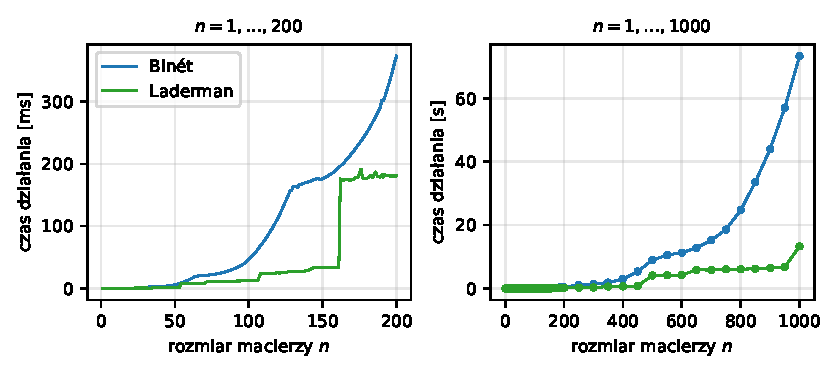
\includegraphics[width=0.86\textwidth]{fig_inv_time.pdf}
\caption{Czas rekurencyjnego odwracania w zależności od rozmiaru macierzy $n$.}
\label{fig:inv-time}
\end{figure}

\begin{figure}[H]
\centering
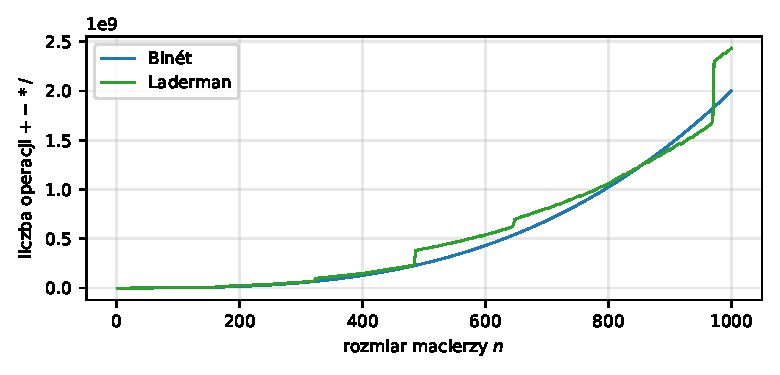
\includegraphics[width=0.78\textwidth]{fig_inv_flops.pdf}
\caption{Liczba operacji zmiennoprzecinkowych rekurencyjnego odwracania dla $n=1,\dots,1000$.}
\label{fig:inv-flops}
\end{figure}

\paragraph{Liczba operacji.} Przy $n=1000$ Binét wykonuje $1{,}999\cdot10^9$ operacji, a Laderman
$2{,}434\cdot10^9$, czyli o 22\% więcej. Laderman ma mniej operacji niż Binét tylko dla 109 ze 1000 wartości $n$.
To ten sam efekt co w zadaniu~1: przy rekurencji do bloków $1\times1$ i $2\times2$ mnożenie Ladermana dla potęg
trójki opłaca się względem Binét'a dopiero od $n=3^9$, bo na każdym poziomie wykonuje 98 dodawań bloków. Nachylenie prostej w skali log-log
(dla $n\ge16$) wynosi 3{,}003 dla Binét'a i 2{,}869 dla Ladermana, blisko teoretycznych $3$ i
$\log_3 23\approx2{,}854$. Stosunek liczby operacji odwracania do mnożenia tą samą metodą ma dla Ladermana
medianę 1{,}17 (dla $n\ge100$), zgodnie z oszacowaniem $\approx1{,}15$, ale waha się od 0{,}73 do 1{,}49.

Na wykresie~\ref{fig:inv-flops} krzywa Ladermana ma skoki, np.\ przy $n=486=2\cdot3^5$ (z $2{,}44\cdot10^8$ do
$3{,}81\cdot10^8$) i $n=972=4\cdot3^5$ (z $1{,}97\cdot10^9$ do $2{,}30\cdot10^9$). Połówki takich $n$ są potęgami
trójki razy mała liczba. Wtedy mnożenie Ladermana dzieli bloki aż do $1\times1$, czyli trafia na swój najdroższy
przypadek: dla $3\times3$ wykonuje 121 operacji zamiast 45. Dla porównania mnożenie $80\times80$ kosztuje u Ladermana
1{,}09 raza tyle co u Binét'a, a $81\times81$ już 2{,}08 raza.

\paragraph{Czas.} Przy $n=1000$ odwracanie trwało 73{,}3\,s z Binétem i 13{,}3\,s z Ladermanem. Laderman jest więc
5{,}5 raza szybszy, mimo że wykonuje więcej operacji. Powód jest ten sam co w zadaniu~1: Binét schodzi z rekurencją
do bloków $1\times1$, więc większość czasu zajmuje tworzenie i kopiowanie małych macierzy, a nie arytmetyka.
Dla porównania samo mnożenie $1000\times1000$ trwało na tym samym komputerze 73{,}0\,s z Binétem i 18{,}0\,s
z Ladermanem (zadanie~1). Odwracanie z Binétem trwa więc tyle co jedno mnożenie, tak jak przewiduje
twierdzenie~\ref{tw:inv-binet}. Nachylenia log-log czasu (dla $n\ge50$) wynoszą 2{,}96 dla Binét'a i 2{,}86 dla
Ladermana.

Skok czasu Ladermana przy $n=162=2\cdot81$ (z 34\,ms do 176\,ms, rysunek~\ref{fig:inv-time}) ma tę samą przyczynę co
skoki liczby operacji. Liczba operacji rośnie tam tylko 1{,}6 raza (z $10{,}2\cdot10^6$ do $16{,}3\cdot10^6$), ale
rekurencja schodzi do bloków $1\times1$, więc wywołań i małych macierzy jest znacznie więcej. Próg przełączenia na
mnożenie klasyczne dla małych bloków usunąłby te skoki, ale zgodnie z zadaniem~1 prowadzimy czystą rekurencję.

\begin{figure}[H]
\centering
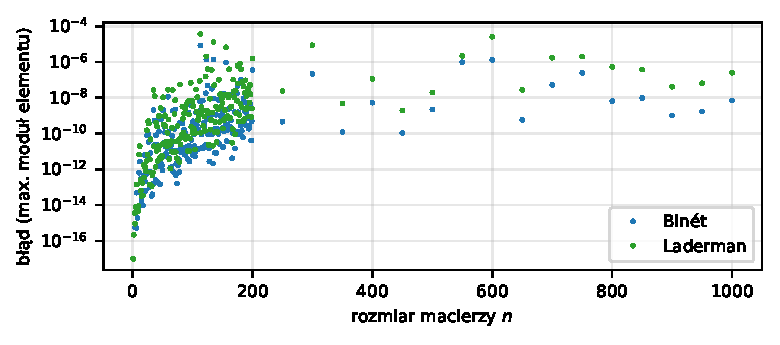
\includegraphics[width=0.78\textwidth]{fig_inv_error.pdf}
\caption{Błąd odwracania $\max_{ij}|(AA^{-1}-I)_{ij}|$ dla macierzy losowych z wykresu~\ref{fig:inv-time}.}
\label{fig:inv-error}
\end{figure}

\paragraph{Dokładność.} Mediana błędu $\max|AA^{-1}-I|$ wynosi $1{,}1\cdot10^{-10}$ dla Binét'a
i $6{,}9\cdot10^{-10}$ dla Ladermana, ale dla niektórych macierzy błąd sięga $10^{-5}$ (najgorzej przy $n=113$:
$8{,}3\cdot10^{-6}$ i $3{,}7\cdot10^{-5}$). Obie metody odwracają te same macierze i skoki błędu wypadają przy
tych samych $n$: współczynnik korelacji logarytmów błędów dla $n=10,\dots,200$ wynosi 0{,}96, a 9 z 10 najgorszych
$n$ jest wspólnych. Błąd zależy więc głównie od macierzy, a nie od metody mnożenia. Laderman ma błąd średnio
(mediana) 6{,}6 raza większy, bo wykonuje więcej dodawań i odejmowań. Przyczyną dużych błędów jest brak wyboru elementu głównego: algorytm dzieli
przez $a_{11}$ i kolejne dopełnienia Schura, a gdy któreś z nich jest bliskie osobliwości, błąd rośnie~\cite{higham}.
Kontrolnie odwróciliśmy macierze diagonalnie dominujące $A+nI$ dla $n=1,\dots,120$: tam błąd nie przekracza
$2{,}4\cdot10^{-15}$ dla obu metod, więc implementacja jest poprawna, a problem dotyczy tylko uwarunkowania.


% 5. FAKTORYZACJA LU
\clearpage
\section{Rekurencyjna faktoryzacja LU}\label{sec:lu}
\todo{pseudokod, dowód poprawności, najważniejsze fragmenty kodu, przykład ręczny LU $3\times3$ (proponujemy tę samą
macierz co w przykładzie odwracania: $L=[1\,0\,0;\,2\,1\,0;\,4\,3\,1]$, $U=[2\,1\,1;\,0\,1\,1;\,0\,0\,2]$),
wykresy czasu i liczby operacji (\texttt{fig\_lu\_time.pdf}, \texttt{fig\_lu\_flops.pdf} z \texttt{make\_plots.py})}

% 6. PODSUMOWANIE
\section{Podsumowanie}
\todo{wnioski po zebraniu wyników odwracania (z Strassenem) i LU}

% LITERATURA
\begin{thebibliography}{9}
\bibitem{strassen} V.~Strassen, \emph{Gaussian elimination is not optimal}, Numerische Mathematik 13 (1969), s.~354--356.
\bibitem{peeling} S.~Huss-Lederman, E.~M.~Jacobson, J.~R.~Johnson, A.~Tsao, T.~Turnbull,
\emph{Implementation of Strassen's algorithm for matrix multiplication}, Supercomputing '96 (1996).
\bibitem{laderman} J.~D.~Laderman, \emph{A noncommutative algorithm for multiplying $3\times3$ matrices using 23
multiplications}, Bulletin of the American Mathematical Society 82 (1976), s.~126--128.
\bibitem{higham} N.~J.~Higham, \emph{Accuracy and Stability of Numerical Algorithms}, wyd.~2, SIAM (2002).
\end{thebibliography}

\end{document}
